\documentclass{beamer}
\usepackage[utf8]{inputenc}

\usepackage[orientation=landscape,size=a0,scale=1.4,debug]{beamerposter}
\usepackage{hyperref}
\usetheme{Boadilla}
\usecolortheme{rose}

% biblatex (requires biber; sudo pacman -S biber)
\usepackage[style=authoryear-ibid]{biblatex} % biblatex
\addbibresource{"./content/bib/bib1.bib"}
\addbibresource{"./content/bib/bib2.bib"}

\usepackage{graphicx}
\graphicspath{ {./content/img/} }

\title[NEXTGEN]{NEXTGEN}
\subtitle{The \textit{\href{https://cryptolog.io}{Secret} Calculating} Technology}
\author[\href{https://nextgen.abdn.ac.uk}{nextgen.abdn.ac.uk} or \href{https://cryptolog.io}{cryptolog.io}]{George Onoufriou, Paul Mayfield, Georgios Leontidis}
\date{\today}

\begin{document}

  \begin{frame}
    \maketitle
    \begin{columns}
      \begin{column}{0.3\textwidth}
        \begin{block}{Fully Homomorphic Encryption as a Service}
          Citation \autocite{gentry2009fully, Goodfellow-et-al-2016}
        \end{block}
      \end{column}
      \begin{column}{0.3\textwidth}
        \begin{block}{Fully Homomorphically Encrypted Pipeline}
          \begin{figure}
            \centering
            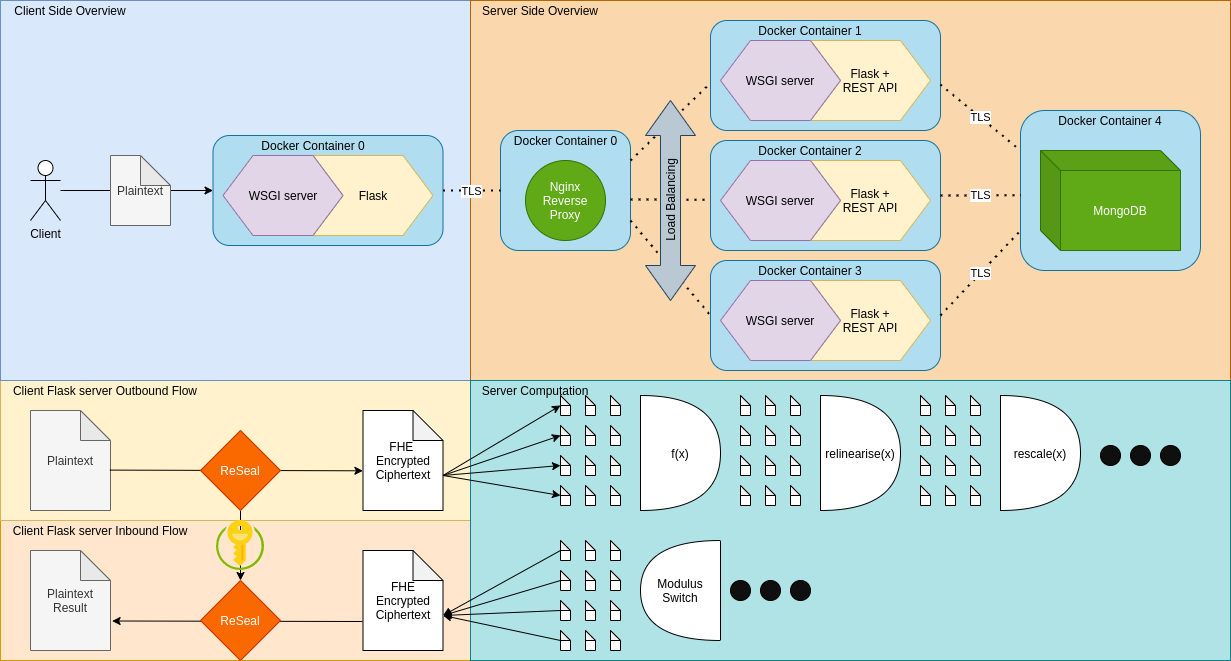
\includegraphics[width=\textwidth]{nextgen.png}
            \caption{Our server-client based pipeline and API for application and evaluation of FHE at some scale.}
            \label{fig:gan}
          \end{figure}
        \end{block}
      \end{column}
      \begin{column}{0.3\textwidth}
        \begin{block}{Fully Homomorphic Encryption as a Service}
        \end{block}
      \end{column}
    \end{columns}

    \begin{columns}
      \begin{column}{0.6\textwidth}
        \begin{block}{Fully Homomorphic Encryption Compatible Simple 1D CNN Computational Graph}
          \begin{figure}
            \centering
            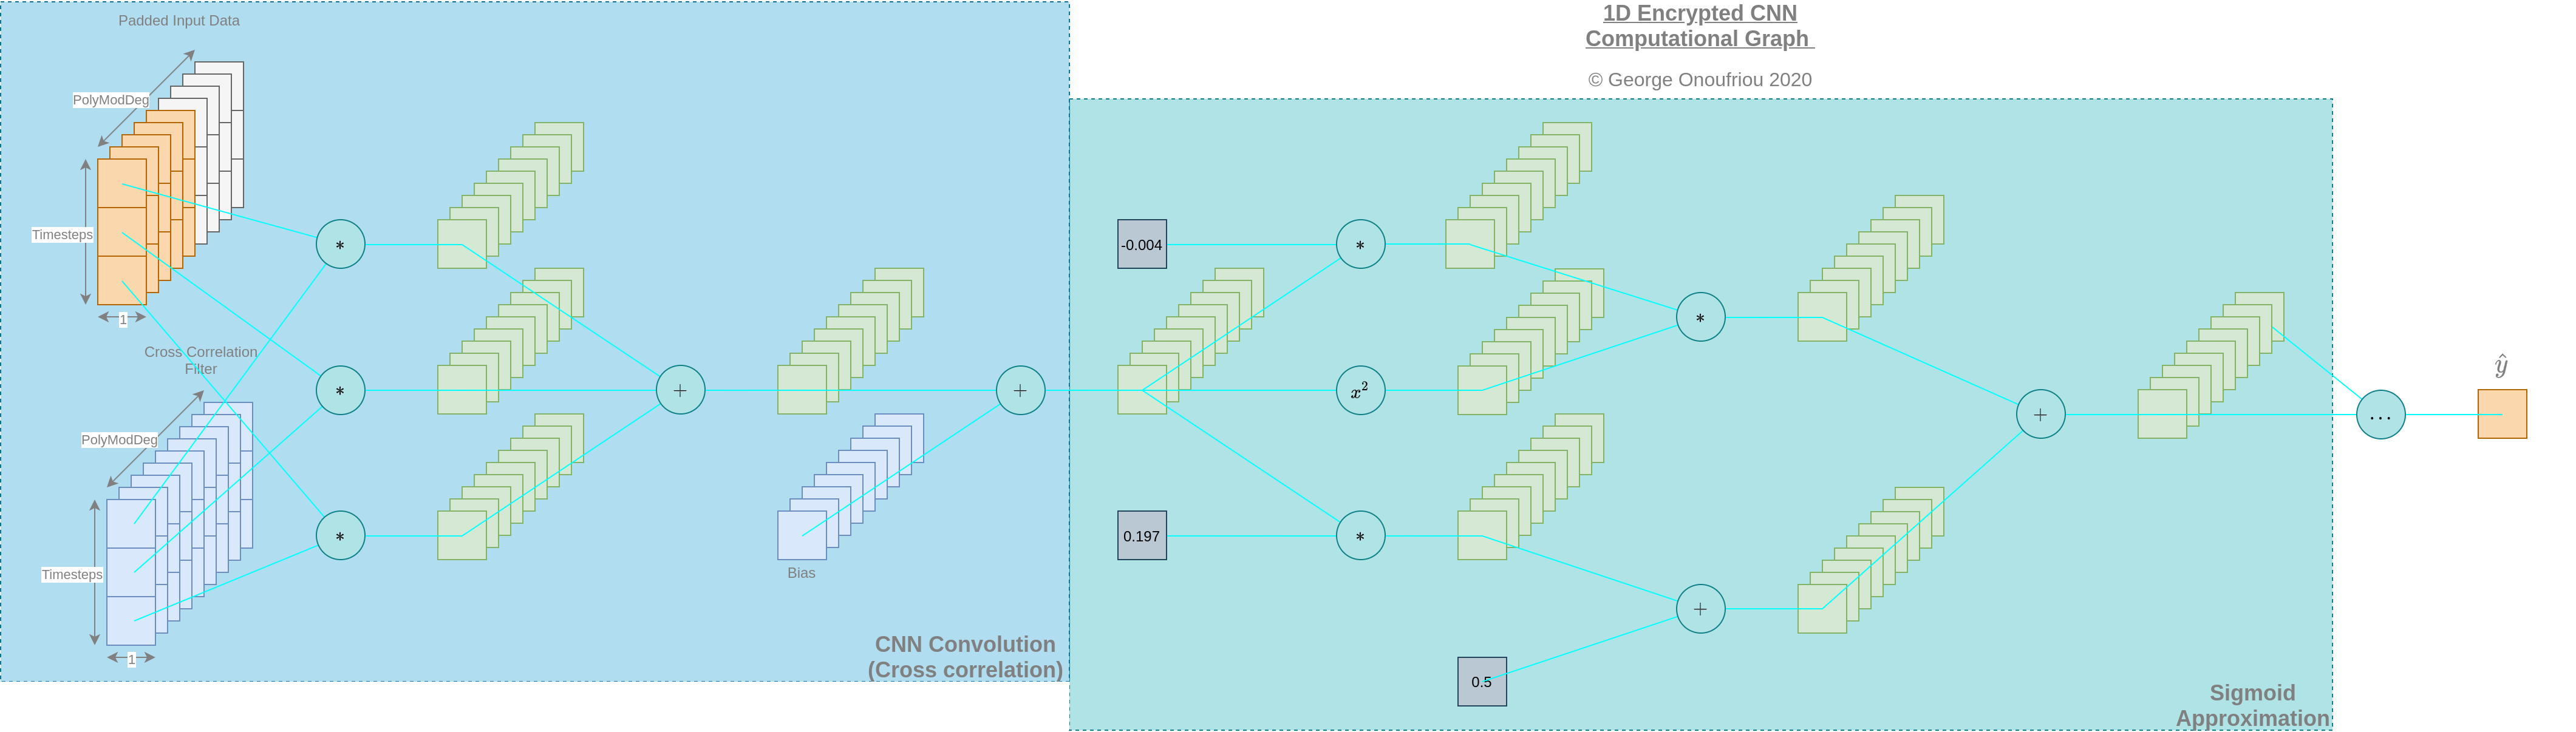
\includegraphics[width=\textwidth]{encrypted_cnn.png}
            \caption{1D CNN computational graph.}
            \label{fig:gan}
          \end{figure}
        \end{block}
      \end{column}
      \begin{column}{0.3\textwidth}
        \begin{block}{Fully Homomorphic Encryption as a Service}
        \end{block}
      \end{column}
    \end{columns}

    \begin{columns}
      \begin{column}{0.3\textwidth}
        \begin{block}{FHE Compatibility and Deep Learning Equation Summary}
          \begin{equation}
            \label{sigmoid}
            \sigma(x) = \frac{1}{1+e^{-x}}
          \end{equation}
          \begin{equation}
            \label{sigmoid_approx}
            \sigma(x) \approx 0.5 + 0.197x + -0.004x^3
          \end{equation}
          \begin{equation}
            \label{cnn_activation}
            a^{<t>}=\sigma(w_{i}^{<t>}x^{<t>}+b_i^{<t>})
          \end{equation}
          \begin{equation}
            \label{gradient}
            \frac{df}{d\sigma} = (1-\sigma(x)) * \sigma(x)
          \end{equation}
          \begin{equation}
            \label{weight_update}
            % learning rate
            w_i^{j+1<t>} = w_i^{j<t>} - (l * \frac{df}{dw_i^{j<t>}})
          \end{equation}
        \end{block}
      \end{column}
      \begin{column}{0.3\textwidth}
        \begin{block}{References}
          \printbibliography
        \end{block}
      \end{column}
    \end{columns}
  \end{frame}
\end{document}
